\documentclass{ieeeaccess}
\usepackage{cite}
\usepackage{amsmath,amssymb,amsfonts}
\usepackage{algorithmic}
\usepackage{graphicx}
\usepackage{textcomp}
\usepackage{balance}
\usepackage{booktabs}
\usepackage{array}
\usepackage{tabularx}

\usepackage{bm}
\makeatletter
\AtBeginDocument{\DeclareMathVersion{bold}
\SetSymbolFont{operators}{bold}{T1}{times}{b}{n}
\SetSymbolFont{NewLetters}{bold}{T1}{times}{b}{it}
\SetMathAlphabet{\mathrm}{bold}{T1}{times}{b}{n}
\SetMathAlphabet{\mathit}{bold}{T1}{times}{b}{it}
\SetMathAlphabet{\mathbf}{bold}{T1}{times}{b}{n}
\SetMathAlphabet{\mathtt}{bold}{OT1}{pcr}{b}{n}
\SetSymbolFont{symbols}{bold}{OMS}{cmsy}{b}{n}
\renewcommand\boldmath{\@nomath\boldmath\mathversion{bold}}}
\makeatother

\def\BibTeX{{\rm B\kern-.05em{\sc i\kern-.025em b}\kern-.08em
    T\kern-.1667em\lower.7ex\hbox{E}\kern-.125emX}}

\begin{document}
\history{Date of publication xxxx 00, 2026, date of current version xxxx 00, 0000.}
\doi{10.1100/ACCESS.2026.0000000}

\title{A Multi-Modal AI Framework for Maritime Security Intelligence from Sentinel-1 SAR: Dark-Vessel Detection, Illegal-Fishing Flagging, and Oil-Spill Assessment}

\author{\uppercase{Navaneeth Bhaskar}\authorrefmark{1} and \uppercase{Shaun Marvell Rodrigues}\authorrefmark{1}}

\address[1]{Nitte (Deemed to be University), NMAM Institute of Technology (NMAMIT), Nitte, Karnataka, India }

%\tfootnote{This work was supported by [funding details].}

\markboth
{Rodrigues \headeretal: IEEE ACCESS}
{Rodrigues \headeretal: IEEE ACCESS}

\corresp{Corresponding author: Shaun Marvell Rodrigues (e-mail: shaunmarvellrodrigues@gmail.com).}


\begin{abstract}
Illegal, unreported and unregulated (IUU) fishing, ``dark'' vessels that disable their Automatic Identification System (AIS), and marine oil discharge are today monitored by separate, stovepiped systems. This paper presents an integrated maritime-security framework that derives all three intelligence products from a single free Sentinel-1 Synthetic Aperture Radar (SAR) scene, imaging through cloud and darkness. The main contributions are: (i)~a hybrid vessel detector that fuses a training-free, resolution-agnostic censored-mean Constant False Alarm Rate (CFAR) stage with a YOLO11m oriented-bounding-box network, so physics-based recall survives the resolution domain gap that degrades learned detectors at Sentinel-1's 10\,m/px resolution, while censoring corrects the classical target-masking failure in dense anchorages; (ii)~transformer-based oil-spill segmentation, benchmarking SegFormer against DeepLabV3+ and U-Net on a public three-part Sentinel-1 oil-spill dataset, together with a cross-distribution robustness analysis on its held-out third part; and (iii)~an AIS cross-checking layer that flags dark vessels and links slicks to candidate source vessels within one georeferenced scene. On the HRSID benchmark, YOLO11m-OBB reaches a mean average precision (mAP@50) of 0.938, with oriented boxes contributing higher gain over horizontal-box baselines, and on a dense Singapore anchorage scene the CFAR stage recovers 257 vessels where the standalone learned detector is inconsistent. SegFormer attains an oil-class intersection-over-union (IoU) of approximately 0.80, sustaining a mean IoU of 0.73 on the deliberately adversarial held-out partition dominated by oil look-alikes. All outputs are georeferenced and served to a lightweight web dashboard, turning raw SAR into actionable maritime-security intelligence that reports oil area, never volume.
\end{abstract}

\begin{keywords}
Maritime surveillance, synthetic aperture radar, Sentinel-1, dark vessel detection, CFAR, oil spill segmentation, SegFormer, AIS fusion.
\end{keywords}

\titlepgskip=-21pt

\maketitle
\section{Introduction}
\label{sec:introduction}

\PARstart{T}{he} world's oceans cover more than seventy percent of the planet and carry the overwhelming majority of global trade, yet they remain among the least observed environments on Earth. This observational gap is exploited at scale. Illegal, unreported and unregulated (IUU) fishing is estimated to account for as much as a fifth of the global catch~\cite{1}, depleting stocks and undermining the economies of coastal states. Vessels engaged in IUU fishing, sanctions evasion, smuggling, or unauthorised operations in restricted waters routinely disable or spoof their Automatic Identification System (AIS) transponders to avoid being tracked, becoming so-called \emph{dark} vessels that are present in the water but absent from the cooperative reporting picture. At the same time, deliberate bilge-water discharge and accidental spills release oil into the marine environment, threatening fisheries, protected habitats and coastal communities. Each of these threats is serious in isolation; together they describe a maritime-security problem that is fundamentally about detecting activity that actively tries not to be seen.

Conventional maritime monitoring is poorly matched to this problem for three reasons. First, it leans heavily on cooperative data: AIS is invaluable when present but is trivially defeated by switching off the transponder, and recent ecological work shows that AIS alone misses a large fraction of the vessels that satellite imagery reveals inside marine protected areas~\cite{2}. Second, the optical satellite imagery that the public associates with ``satellite surveillance'' is blind at night and through cloud, and is typically months to years stale---unusable for time-critical, all-weather operations. Third, the capabilities that do exist tend to be deployed as separate, stovepiped systems---one tool for vessel detection, another for fishing analysis, another for pollution monitoring---so that the connections between them, such as linking a fresh oil slick to a nearby non-broadcasting vessel, are never made automatically. Spaceborne Synthetic Aperture Radar (SAR) addresses the first two limitations directly: as an active microwave sensor it images day and night and penetrates cloud, and recent large-scale studies have demonstrated that SAR can map industrial activity at sea that is invisible to AIS~\cite{3}. What has been missing is an integrated, reproducible system that turns a single SAR scene into a complete maritime-security picture.

These limitations establish the need for the approach taken in this work: an integrated system built entirely on Sentinel-1, the freely available European C-band SAR mission, whose Interferometric Wide-swath Ground Range Detected (IW GRD) product images a 250\,km swath at roughly 10\,m/px with a six-day repeat cycle, and whose constellation is being renewed by Sentinel-1C and Sentinel-1D, so the data format on which our pipeline depends will persist. Oil slicks and ships are extracted from the \emph{same} georeferenced scene, so they are automatically co-registered and time-aligned, and AIS need only be matched to the scene's known acquisition timestamp rather than to a live feed. From one scene the framework (i)~detects every vessel using a training-free censored-mean Constant False Alarm Rate (CFAR) detector paired with a YOLO11m oriented-bounding-box network trained on the HRSID dataset~\cite{4}; (ii)~segments oil slicks with a SegFormer~\cite{5} transformer trained on the Sentinel-1 oil-spill dataset of Trujillo-Acatitla~\textit{et~al.}~\cite{6}, benchmarked against DeepLabV3+ and U-Net; (iii)~cross-checks detections against historical AIS to flag dark vessels; (iv)~applies a rule-based zone-violation and risk-scoring layer that links slicks to candidate responsible vessels; and (v)~serves all outputs as georeferenced layers to a lightweight web dashboard.

The contributions are framed around reproducible, code-verified findings rather than headline benchmark numbers. We show that a censored-mean CFAR detector provides \emph{resolution-agnostic} ship detection at Sentinel-1's 10\,m/px scale, where the HRSID-trained network (mAP@50 of $0.938$) suffers a domain gap, and that the censoring step corrects the classical target-masking failure that suppresses dim vessels beside bright ones in dense anchorages. We benchmark three segmentation architectures on a public three-part Sentinel-1 oil-spill dataset, reaching a validation oil-class IoU of $\approx0.80$ with SegFormer, and complement the benchmark with a cross-distribution robustness analysis on the deliberately adversarial held-out partition, in which SegFormer degrades least. We further analyse the resolution and cross-region domain gaps that bound generalisation (identifying xView3-SAR as the principled remedy for the former) and deliver the whole pipeline as one operational system rather than a collection of disconnected models. Throughout, we are careful not to overclaim: a recently published ``SOTA'' oil model whose code was never released could not be benchmarked, so we train and report SegFormer directly, and we stress that SAR yields oil \emph{area/extent}, never volume.

\section{Related Works}

Research relevant to this framework spans three threads: SAR vessel detection (covering both classical Constant False Alarm Rate detectors and learned networks), SAR oil-spill segmentation, and the fusion of SAR detections with AIS to reveal dark vessels. We review ten representative works, emphasising publications from 2022 onward, and position our design against each.

The largest labelled benchmark for SAR vessel and infrastructure detection is xView3-SAR, introduced by Paolo~\textit{et~al.}~\cite{7}: nearly one thousand analysis-ready Sentinel-1 scenes that are on average $29{,}400\times24{,}400$ pixels, together with bathymetry and wind-state layers. The associated international challenge brought the problem of dark, AIS-absent vessels to the machine-learning community and produced models that have since been deployed operationally against illegal fishing. Crucially for our work, xView3 is Sentinel-1 Interferometric Wide-swath imagery at roughly the same medium ($\sim$10--20\,m/px) resolution at which our pipeline operates; we therefore identify fine-tuning on xView3-SAR as the principled remedy for the resolution domain gap that affects our HRSID-trained detector, and treat it as future work rather than a component of the present system.

Among learned detectors, AMANet~\cite{8} is an adaptive multi-hierarchical attention network that fuses information across adjacent feature layers and adaptively combines channel features, improving average precision on the SSDD and HRSID benchmarks over its baseline. It is representative of the strong attention-augmented CNN detectors that define recent HRSID performance. Like the great majority of SAR ship-detection papers, however, AMANet is trained and evaluated at HRSID's native high resolution, where a $100$\,m vessel spans tens to hundreds of pixels, and it does not address the distribution shift that arises at $10$\,m/px Sentinel-1 IW resolution---the regime in which our pipeline must operate.

The YOLO lineage remains the reference point on these benchmarks: AC-YOLO~\cite{9}, a lightweight detector built on YOLO11 by He~\textit{et~al.}, integrates an ACmix attention module, a CCFM feature-fusion neck, and an MPDIoU regression loss, raising mAP by $1.5\%$ on HRSID and $1.2\%$ on SSDD while reducing parameters by roughly a third. This confirms that YOLO11-class architectures are the current high-water mark for SAR ship detection and directly motivates our choice of a YOLO11m oriented-bounding-box backbone. As with AMANet, however, the gains are demonstrated at training resolution; architectural refinement alone does not close the medium-resolution inference gap, which is why our system pairs the learned detector with a physics-based detector rather than relying on it alone.

Closest in spirit to our hybrid detector, Wen~\textit{et~al.}~\cite{10} embedded a sub-network that learns classical CFAR features inside YOLOv5s, enhancing sensitivity to low-contrast targets. Our design differs in an important respect: rather than folding CFAR into the learned detector as a trainable feature, we retain a separate, \emph{training-free} censored-mean CFAR stage that is resolution-agnostic and gates the YOLO detections, so the physics-based component requires no retraining when the sensor or pixel size changes.

On the purely classical side, Zhang~\textit{et~al.}~\cite{11} developed an improved superpixel-level CFAR (SP-CFAR) for high-resolution SAR, replacing the rectangular clutter window with superpixels so that the detection threshold is estimated from pure-clutter regions, which markedly improves inshore and densely packed ship detection. SP-CFAR is effectively the non-deep-learning state of the art for dense scenes, but a full superpixel pass over a multi-thousand-pixel scene is comparatively slow and would conflict with the absolute-threshold land mask our pipeline relies on. We therefore adopt censored-mean CFAR (CMLD), a faster member of the same robustness family, which recovers most of SP-CFAR's benefit by censoring bright interferers from the clutter estimate while preserving cell-averaging speed.

Turning to oil-spill segmentation, Wu~\textit{et~al.}~\cite{12} proposed a compositional detector that pairs YOLOv8 with an adapted Segment Anything Model, converting detected boxes into masks and fusing them through an ordered-mask module. This SAM-based direction is precisely the lineage of the recently announced ``OilSAM2'' model we had hoped to benchmark; because that model's code was never publicly released, our system instead uses a directly trained SegFormer, and we report results as SegFormer rather than as the unavailable state of the art.

Data scarcity is a chronic obstacle in SAR oil-spill segmentation, and Moon~\textit{et~al.}~\cite{13} attack it using diffusion-generated synthetic imagery and knowledge distillation over soft labels, improving minority-class performance without a pre-trained teacher. Their approach is complementary to the look-alike hard-negative upsampling we employ and points to a promising augmentation route for closing the validation-to-test gap we report.

Most directly relevant to our central empirical finding, Juarez~\textit{et~al.}~\cite{14} studied cross-domain oil-spill segmentation and reported that a model trained on Mediterranean data degrades from $67.8\%$ to $51.8\%$ mean IoU when transferred to a Peruvian domain, recovering up to $+6$ mIoU with morphological region perturbation and synthetic SAR generation. Their result independently corroborates the large cross-distribution drop we observe and reinforces our argument that a genuinely disjoint evaluation is essential when characterising oil-segmentation robustness.

On the fusion side, Paolo~\textit{et~al.}~\cite{3} mapped global industrial activity at sea by combining Sentinel-1 SAR, AIS, and three deep convolutional networks for object detection, length estimation, and vessel classification, finding that $72$--$76\%$ of the world's industrial fishing vessels are absent from public tracking. This study is the methodological anchor for the principle that SAR reveals activity invisible to AIS; our framework operationalises the same detect-then-cross-check logic at single-scene granularity and layers integrated risk scoring on top.

Complementarily, Raynor~\textit{et~al.}~\cite{2} combined AIS with SAR to study fishing inside strictly protected marine areas and found that AIS missed close to $90\%$ of the fishing vessels that SAR detected in coastal zones. This quantifies precisely why AIS-only monitoring is insufficient and motivates the dark-vessel flagging and zone-violation logic at the heart of our risk layer.

Taken together, these works advance individual components---learned or classical vessel detection, oil-spill segmentation, and AIS--SAR fusion---but none integrates detection, oil segmentation, AIS-based dark-vessel discrimination, and rule-based risk scoring into a single operational pipeline driven by one freely available sensor. That integration, together with the practical systems lessons we document, is the contribution of this paper.

\section{Methodology}

This section describes the end-to-end framework, from raw Sentinel-1 imagery to the georeferenced intelligence products consumed by the dashboard. The design is modular: two independent perception branches---vessel detection and oil-spill segmentation---each apply the SAR preprocessing matched to their own training distribution (Section~\ref{subsec:prep}), and their outputs are fused with AIS into dark-vessel flags, zone violations, and risk scores. Fig.~\ref{fig:methodology} presents the overall block diagram.

A Sentinel-1 scene is first converted to model-ready tensors by the per-branch preprocessing described alongside the datasets (Section~\ref{subsec:data}). The vessel branch (Section~\ref{subsec:ships}) runs a training-free censored-mean CFAR detector that is robust to the medium-resolution domain gap, and confirms its candidates with an oriented-box YOLO11m network. The oil branch (Section~\ref{subsec:oil}) segments slicks with a SegFormer transformer using a whole-scene-resize inference path that matches the training field of view. The fusion layer (Section~\ref{subsec:fusion}) cross-checks detections against AIS positions interpolated to the acquisition time to flag dark vessels, links slicks to nearby vessels as candidate sources, and computes security and environmental risk scores. All geometry is carried in the scene's affine transform so that every output is georeferenced in WGS84.

\subsection{Datasets and Preprocessing}
\label{subsec:data}

The framework is trained on two public SAR datasets, summarised in Table~\ref{tab:datasets}. Vessel detection uses HRSID~\cite{4}, a high-resolution SAR ship-detection dataset of $5{,}604$ image chips ($800\times800$\,px) containing $16{,}951$ ship instances; we use the standard split of $3{,}642$ training and $1{,}962$ test images, augmented with $400$ pure-background negative chips as hard negatives. HRSID imagery is considerably finer in ground resolution than the $\sim$10\,m/px Sentinel-1 Interferometric Wide-swath (IW) scenes on which the deployed system operates, and this resolution difference is the source of the ship-detection domain gap addressed in Section~\ref{subsec:ships}. Oil-spill segmentation uses the three-part Sentinel-1 SAR oil-spill dataset of Trujillo-Acatitla~\textit{et~al.}~\cite{6} (backscatter $\sigma^0$ in decibels, dual VV/VH polarisation, $2048\times2048$\,px, C-band). Following the dataset's intended protocol, Parts~I and~II ($\approx2{,}570$ oil, look-alike, and clean-sea images) form the train/validation pool, while Part~III ($450$ images, evenly split across oil, look-alike, and clean-sea) is held out as a disjoint test set, which Section~\ref{sec:results} uses for a cross-distribution robustness analysis. At deployment the system ingests live Sentinel-1 C-band IW GRD scenes (VV/VH, $\sim$10\,m/px).

\label{subsec:prep}%
The two datasets differ in source format---decibel GeoTIFFs for the oil segmenter versus 8-bit log-scaled display chips for the vessel detector---so each perception branch applies the preprocessing that matches \emph{its own} training distribution, identically at training and at inference time to avoid train/serve skew. The two chains are deliberately distinct and are described in turn.

The oil branch ingests the Sentinel-1 oil scenes as the backscatter coefficient $\sigma^0$ in decibels, which is first converted to linear power,
\begin{equation}
x_{\text{lin}} = 10^{\,x_{\text{dB}}/10}
\label{eq:dblin}
\end{equation}
Multiplicative SAR speckle is suppressed with a $7\times7$ Lee filter, which blends the local mean $\bar{x}$ with the observed value according to the local signal-to-noise ratio,
\begin{equation}
\hat{x} = \bar{x} + W\,(x - \bar{x}),
\qquad
W = \frac{\max(\sigma^2 - \sigma_n^2,\,0)}{\sigma^2 + \epsilon}
\label{eq:lee}
\end{equation}
where $\bar{x}$ and $\sigma^2$ are the mean and variance in the local window and $\sigma_n^2$ is the scene-level noise variance; in homogeneous sea $W\!\to\!0$ (strong smoothing) while over bright targets $W\!\to\!1$ (edges preserved). Each band is then normalised by clipping at its $99.5$th percentile $q_{99.5}$ (computed over valid, non-\textsc{nodata} pixels) and scaling to the unit interval,
\begin{equation}
x_{\text{norm}} = \mathrm{clip}\!\left(\frac{x}{q_{99.5}},\,0,\,1\right)
\label{eq:pctnorm}
\end{equation}
after which the two polarisations are stacked as $[\text{VV},\text{VH},\text{VH}]$, resized to $512\times512$, and ImageNet-normalised. This exact sequence is applied both to the training tiles and to the whole scene at inference (Section~\ref{subsec:oil}).

The vessel branch, by contrast, is trained on HRSID chips that are already 8-bit, log-scaled display images (dark sea near $0$, bright ships near $255$), so the YOLO detector is trained on them directly, scaling $0$--$255$ to $[0,1]$ without the dB$\to$linear or Lee steps---applying a Lee filter here would blur the few-pixel ship signatures the detector must learn. To present a live Sentinel-1 scene in the same distribution, each polarisation is instead normalised with a fixed decibel window (not a speckle filter),
\begin{equation}
x_{\text{norm}} = \mathrm{clip}\!\left(\frac{x_{\text{dB}} - \ell}{h - \ell},\,0,\,1\right)
\label{eq:dbwin}
\end{equation}
with windows $[\ell,h]=[-25,0]$\,dB for VV and $[-30,-10]$\,dB for VH; this maps open sea to a mid-grey level and ships ($-5$ to $0$\,dB) to near-white, reproducing the HRSID appearance the detector learned. The CFAR stage operates separately on linear VH power $P=10^{\sigma^0/10}$ (Section~\ref{subsec:ships}).

One polarisation choice is shared by both branches: the cross-polarised VH channel is duplicated in the $[\text{VV},\text{VH},\text{VH}]$ stack, because VH has $10$--$15$\,dB lower sea clutter than co-polarised VV, giving a much higher target-to-clutter ratio for ships and the strongest contrast for oil, while VV supplies sea-state context that helps reject look-alikes. This reflects a physical asymmetry the system exploits throughout: oil is polarisation-sensitive (its signal lives in VH),\footnote{The two oil-dataset bands are labelled VV/VH, but band~1 (nominal VV) is measurably darker than band~2 (nominal VH)---the reverse of the usual ocean co/cross-pol ordering---so the labels may be swapped or the scenes simply low-VV. This does not affect training: the informative channel, the one carrying the $\approx\!9$\,dB oil contrast, is band~2 regardless of its nominal label.} whereas ships are polarisation-robust bright point targets.

\subsection{Vessel Detection: Censored-Mean CFAR and YOLO11m-OBB}
\label{subsec:ships}

The learned detector is trained on high-resolution HRSID imagery but must run on $10$\,m/px Sentinel-1 scenes, where a $100$\,m vessel spans only about ten pixels, so a single learned detector alone is unreliable. We therefore make a training-free, resolution-agnostic Constant False Alarm Rate (CFAR) detector the primary stage and use the learned network for confirmation and oriented geometry. Operating on linear VH power $P$, CFAR compares each cell under test against an estimate of the local sea clutter drawn from a training annulus $\mathcal{R}$ (an outer window of half-width $T$ minus a guard region of half-width $G$). The annulus mean and standard deviation are
\begin{equation}
\mu_{\mathcal{R}} = \frac{1}{|\mathcal{R}|}\sum_{i\in\mathcal{R}} P_i,
\qquad
\sigma_{\mathcal{R}} = \sqrt{\,\overline{P^2_{\mathcal{R}}} - \mu_{\mathcal{R}}^2\,}
\label{eq:ringstats}
\end{equation}
Plain cell-averaging CFAR uses $\mu_{\mathcal{R}}$ directly, but in dense anchorages or near bright ocean fronts a second vessel inside the annulus inflates this mean and masks nearby dimmer targets. We instead use \emph{censored-mean} CFAR (CMLD): cells brighter than $\mu_{\mathcal{R}}+\kappa\,\sigma_{\mathcal{R}}$ are treated as interferers and excluded, and the clutter level is re-estimated over the surviving pure-clutter set $\mathcal{K}$,
\begin{equation}
\mathcal{K} = \{\,i\in\mathcal{R} : P_i \le \mu_{\mathcal{R}} + \kappa\,\sigma_{\mathcal{R}}\,\},
\qquad
\hat{\mu} = \frac{1}{|\mathcal{K}|}\sum_{i\in\mathcal{K}} P_i
\label{eq:censor}
\end{equation}
A pixel is declared a candidate target when its power exceeds the adaptive threshold
\begin{equation}
P_{\text{CUT}} > \alpha\,\hat{\mu}
\label{eq:cfarthresh}
\end{equation}
with detector parameters $G=5$, $T=20$, scale factor $\alpha=20$, and censoring factor $\kappa=3$. Connected components smaller than $14$ pixels (isolated speckle) are discarded, and a land/water mask---a $-18$\,dB threshold on the mean of the two polarisations followed by a large morphological opening, so that only solid landmasses survive while bright sea texture and ship-sized returns are removed---suppresses coastal and urban false alarms. In parallel, a YOLO11m oriented-bounding-box network trained on HRSID detects ships and returns rotated boxes $(c_x,c_y,w,h,\theta)$ that supply vessel orientation and length. To suppress YOLO false positives on sea speckle, a YOLO detection is retained only if it agrees with a CFAR candidate within a gate radius $r_g=15$\,px; the final detection set merges the confirmed oriented boxes with the CFAR detections that YOLO did not already cover,
\begin{equation}
\mathcal{D} = \mathcal{D}_{\text{YOLO}}^{\text{conf}} \;\cup\;
\{\,d \in \mathcal{D}_{\text{CFAR}} : \min_{y\in\mathcal{D}_{\text{YOLO}}^{\text{conf}}}
\lVert d - y\rVert > r_m\,\}
\label{eq:merge}
\end{equation}
with merge radius $r_m=10$\,px. Thus CFAR provides resolution-robust recall while YOLO contributes precise oriented geometry for the vessels it can resolve. The detector is trained from the HRSID checkpoint with random scale augmentation ($0.1\times$--$1.9\times$) so that it also sees ships at the $5$--$15$\,px sizes typical of Sentinel-1 IW.

\subsection{Oil-Spill Segmentation}
\label{subsec:oil}

Oil slicks are segmented with a SegFormer transformer (MiT-b5 backbone), benchmarked against DeepLabV3+ and U-Net baselines. Oil pixels constitute under $2\%$ of a scene, so a plain cross-entropy objective collapses to predicting ``all sea.'' We therefore train with a combined Dice--Focal loss,
\begin{equation}
\mathcal{L} = \lambda_f\,\mathcal{L}_{\text{focal}} + \lambda_d\,\mathcal{L}_{\text{dice}}
\label{eq:loss}
\end{equation}
where the class-weighted focal term down-weights easy background pixels,
\begin{equation}
\mathcal{L}_{\text{focal}} = -\frac{1}{N}\sum_{n=1}^{N} w_{c_n}\,(1 - p_{t,n})^{\gamma}\,\log p_{t,n}
\label{eq:focal}
\end{equation}
and the Dice term directly optimises region overlap,
\begin{equation}
\mathcal{L}_{\text{dice}} = 1 - \frac{1}{C}\sum_{c=1}^{C}
\frac{2\sum_n p_{c,n}\,g_{c,n} + s}{\sum_n p_{c,n} + \sum_n g_{c,n} + s}
\label{eq:dice}
\end{equation}
with focusing parameter $\gamma=2$, smoothing constant $s=1$, equal weighting $\lambda_f=\lambda_d=0.5$, and inverse-frequency class weights $w_c$ that compensate for the oil-pixel scarcity. Look-alike hard negatives (low-wind patches, biogenic slicks) are over-sampled during training so the model learns that ``dark $\neq$ oil.'' At inference, the whole scene is resized to $512\times512$ before the network and the prediction is upsampled back---reproducing the field of view the model was trained on, which avoids a $4\times$ resolution skew that native-chip inference would otherwise introduce. A pixel is labelled oil when its oil-class probability exceeds a threshold,
\begin{equation}
M(x,y) = \mathbf{1}\!\left[\,\mathrm{softmax}\big(f_\theta(I_{512})\big)_{\text{oil}}(x,y) > \tau\,\right]
\label{eq:mask}
\end{equation}
where the threshold $\tau\in[0.30,\,0.35]$ is set below the argmax value of $0.5$ because the model under-predicts oil (favouring precision over recall on look-alikes). Segmentation quality is measured by the oil-class Intersection-over-Union,
\begin{equation}
\text{IoU} = \frac{TP}{TP + FP + FN}
\label{eq:iou}
\end{equation}
and the binary mask is vectorised into lon/lat polygons whose extent is reported as a ground area
\begin{equation}
A = \frac{s^2}{10^6}\sum_{p}\,[\,M_p = 1\,] \quad [\text{km}^2]
\label{eq:area}
\end{equation}
with $s$ the ground sampling distance in metres. We emphasise that this is the slick's surface \emph{area}; SAR cannot measure slick thickness, so no oil volume is reported.

\subsection{AIS Fusion and Risk Scoring}
\label{subsec:fusion}

Every detection's pixel coordinates $(x,y)$ are mapped to geographic coordinates through the scene's affine transform,
\begin{equation}
\text{lon} = c + a\,x + b\,y, \qquad \text{lat} = f + d\,x + e\,y
\label{eq:affine}
\end{equation}
The pipeline implements AIS cross-checking by interpolating historical AIS positions to the scene's exact acquisition timestamp and matching each SAR detection to the nearest broadcasting vessel; a detection with no AIS neighbour within a gate radius $r_{\text{match}}=500$\,m is flagged as a dark vessel,
\begin{equation}
\text{dark}(d) = \mathbf{1}\!\left[\,\min_{j}\,\lVert p_d - p^{\text{AIS}}_j\rVert > r_{\text{match}}\,\right]
\label{eq:dark}
\end{equation}
Historical AIS suitable for this matching is publicly distributed by national authorities: the United States Coast Guard archive is served through NOAA's MarineCadastre platform as daily CSV files covering U.S. coastal waters from 2009 onward, and the Danish Maritime Authority publishes an equivalent open historical feed for Danish waters. The pipeline ingests such records as standard position/timestamp tables, interpolating each vessel's track to the scene's acquisition time before matching, and the same interface accepts commercial all-vessel archives for regions outside public coverage. The fusion layer then links each oil slick to nearby dark vessels as candidate responsible parties: a slick with centroid $c_s$ and a dark vessel at $p_v$ are associated when
\begin{equation}
\lVert c_s - p_v \rVert \le R
\label{eq:fuse}
\end{equation}
within a configurable search radius $R$. Optionally, when Exclusive Economic Zone or Marine Protected Area polygons are supplied, a vessel falling inside a no-take or restricted zone additionally raises a zone violation. These signals combine into bounded security and environmental risk scores,
\begin{align}
S ={}& \min\!\big(100,\; 40\cdot\mathbf{1}[\text{dark}] + 25\cdot\mathbf{1}[\text{dark}\wedge\text{MPA}] \nonumber\\
     & \qquad\; + 20\cdot\mathbf{1}[\text{IUU}] + 15\cdot\mathbf{1}[\text{anomaly}]\big)
\label{eq:secrisk}\\
E ={}& \min\!\big(100,\; 40\,\sigma_{\text{sev}} + 25\cdot\mathbf{1}[\text{near coast}] \nonumber\\
     & \qquad\; + 20\cdot\mathbf{1}[\text{near MPA}] + \delta_{\text{drift}}\big)
\label{eq:envrisk}
\end{align}
where $\sigma_{\text{sev}}\in[0,1]$ is the area-derived spill severity and $\delta_{\text{drift}}$ rewards short drift-to-shore times. Both scores are built from explicit, bounded rule terms with fixed weights, so every score is directly traceable to the observable factors---AIS absence, restricted-area presence, proximity to a slick, and slick size---that produced it.

\subsection{Experimental Setup}
\label{subsec:setup}

The three vessel detectors were trained on HRSID for $50$ epochs using the standard $3{,}642$/$1{,}962$ train/test split ($5{,}922$ ship instances in the test set) on dual NVIDIA T4 GPUs. The three oil segmenters were trained for $50$ epochs on Parts~I+II of the Trujillo-Acatitla dataset (an $\approx85$/$15$ train/validation split) on an NVIDIA H100, and then evaluated on the held-out Part~III test set. Detection quality is reported as precision, recall, $F_1$, and mean average precision at IoU~$0.50$ (mAP@50) and averaged over $0.50$--$0.95$ (mAP@50-95). Segmentation quality is reported as the oil-class Intersection-over-Union (OilIoU) and the mean IoU over both classes (mIoU); the \emph{validation} figures (same distribution as training) serve as the primary benchmark, while the disjoint Part~III set drives the cross-distribution robustness analysis of Section~\ref{subsec:robust}. AIS tracks for the study scenes were emulated at the scene acquisition timestamps; the matching pipeline of Section~\ref{subsec:fusion} operates identically when a provider feed such as MarineCadastre is connected.

\section{Results and Discussion}
\label{sec:results}

This section reports the quantitative benchmarks for the two perception branches, the comparison between the classical and learned detectors at operational resolution, and qualitative outputs of the integrated system, all obtained under the experimental setup of Section~\ref{subsec:setup}.

\subsection{Vessel Detection Benchmark}

Table~\ref{tab:ships} compares the three detectors on the HRSID test set, and Fig.~\ref{fig:shipcurves} shows the validation mAP@50 over training, where the oriented-box model holds a visible margin over both horizontal-box models for essentially the whole run. The oriented-bounding-box model, YOLO11m-OBB, is the clear winner, reaching an mAP@50 of $0.938$ and mAP@50-95 of $0.688$ with the highest recall ($0.873$).

The most instructive result is not the winner's margin but \emph{where} it comes from. The $2026$-generation horizontal-box detector YOLO26m ($0.908$ mAP@50) is statistically indistinguishable from the $2023$ horizontal-box baseline YOLOv8m ($0.910$)---three years of architectural advancement produce no meaningful gain on this task. Adding oriented bounding boxes, on the other hand, lifts mAP@50 by $+2.8$ points ($0.910\!\rightarrow\!0.938$) and recall by $+5.1$ points. For elongated SAR ship targets at arbitrary headings, a tightly fitted rotated box excludes the speckle-dominated background that a horizontal box would enclose, and this geometric prior is worth far more than a newer detection head.

The precision--recall profiles in Table~\ref{tab:ships} reinforce the choice. YOLO26m attains the best precision ($0.926$) but the lowest recall ($0.802$)---the signature of a conservative detector---whereas the oriented-box model pairs near-identical precision ($0.920$) with the highest recall ($0.873$). In maritime surveillance the asymmetry matters: a missed dark vessel is unrecoverable, while a false alarm is subsequently filtered by the CFAR cross-check of Section~\ref{subsec:ships}, so the recall-leaning profile is operationally preferable. The gain is also economical---at $2.42$\,h on dual T4 GPUs, the oriented-box model trains between the two horizontal-box baselines, so the $+2.8$-point improvement carries no meaningful compute cost. We therefore adopt YOLO11m-OBB as the learned detector. Its oriented predictions are illustrated in Fig.~\ref{fig:shippred}.

\subsection{Resolution-Robust Detection with Censored-Mean CFAR}

The HRSID benchmark above is measured at HRSID's native high resolution. At the $\sim$10\,m/px resolution of live Sentinel-1 IW scenes, the same YOLO detector degrades sharply because ships shrink to $5$--$15$ pixels, far below the sizes seen in training. Table~\ref{tab:cfar} reports detection counts on a dense Sentinel-1 scene of the Singapore Eastern Anchorage ($\sim$10\,m/px), where the training-free censored-mean CFAR detector recovers the most vessels while the standalone learned detector is inconsistent.

CFAR succeeds here precisely because it is adaptive to local clutter statistics rather than to a learned object scale. The censoring step is what makes it reliable in dense traffic: in a controlled masking test with a dim vessel adjacent to a bright one over calm sea, plain cell-averaging CFAR inflated its threshold to $1.135$ and \emph{missed} the dim target, whereas censored-mean CFAR held the threshold at $0.502$ and detected it. The learned detector can itself be partially adapted to this regime: fine-tuning YOLO11m-OBB with aggressive scale augmentation ($0.1$--$1.9\times$) trades a little HRSID accuracy---its test mAP@50 regresses from $0.938$ to $0.910$---for the ability to fire on the $5$--$15$-pixel vessels typical at $10$\,m/px; because no labelled ground truth exists for the Sentinel-1 scenes, this robustness gain is shown qualitatively rather than as a benchmark number. Even so, CFAR remains the more reliable recall source at this resolution, which is why it is kept as the primary detector while YOLO supplies oriented geometry. The fusion policy in Section~\ref{subsec:ships} keeps CFAR's recall while attaching YOLO's oriented geometry to the vessels it can resolve. For a qualitative view we use a cleaner open-water scene, the Strait of Malacca, where detections sit on open sea away from coastal clutter; it is shown in Fig.~\ref{fig:cfarpred}.

\subsection{Oil-Spill Segmentation Benchmark}

Table~\ref{tab:oil} benchmarks four model variants across three architectures---U-Net, DeepLabV3+, and SegFormer at the b4 and b5 backbone sizes---and Fig.~\ref{fig:oilcurves} shows the validation oil-class IoU over training. SegFormer is the strongest architecture: SegFormer-b4 attains the best validation OilIoU of $0.799$, with b5 essentially tied at $0.795$, ahead of DeepLabV3+ ($0.773$) and U-Net ($0.750$). The transformer's margin is present throughout the training run rather than only at the final epoch, and it comes at acceptable cost---SegFormer-b5 trains in $1$\,h\,$15$\,m on the H100, against $44$--$45$\,m for the CNN baselines. A qualitative segmentation result on a held-out scene is shown in Fig.~\ref{fig:oilpred}.

\subsection{Cross-Distribution Robustness Analysis}
\label{subsec:robust}

To probe behaviour beyond the training distribution, all four models are additionally evaluated on the held-out Part~III partition, whose $450$ scenes are deliberately adversarial: a full third are look-alikes (low-wind patches, biogenic slicks) that mimic oil's dark signature. Table~\ref{tab:oil} lists these figures alongside the validation benchmark. Every architecture degrades on this stress set---the strict oil-class IoU falls to $0.48$ for SegFormer while the mean IoU remains at $0.73$---and SegFormer degrades least ($-0.31$, against $-0.42$ for DeepLabV3+ and $-0.38$ for U-Net), so its advantage is one of robustness as well as accuracy. The degradation is driven by the look-alike scenes triggering false positives on the strict oil class, and its magnitude closely matches the independent cross-domain drop reported by Juarez~\textit{et~al.}~\cite{14}, which situates our stress-set figures squarely within the behaviour the literature documents for distribution shift in SAR oil segmentation.

A post-hoc threshold sweep over the oil-class probability ($\tau$ from $0.30$ to $0.80$) characterises the error mode further. At the default argmax operating point the model is markedly precision-favouring: oil-pixel precision on the stress set is high ($0.88$--$0.90$) while recall is only $\approx0.51$, i.e., the dominant failure is missed faint oil rather than hallucinated oil. Lowering the threshold to its optimum at $\tau=0.30$ raises the SegFormer-b5 stress-set OilIoU only marginally, from $0.484$ to $0.490$ ($+0.006$)---threshold tuning cannot close the distribution gap, because the missing accuracy lies in the data distribution rather than in the operating point. This motivates the cross-region training data identified as future work in Section~\ref{sec:discussion}, and it fixes the deployed inference threshold in the $\tau\in[0.30,0.35]$ recall band of \eqref{eq:mask}.

Per-scene behaviour on the stress set is also more encouraging than the aggregate suggests. On individual Part~III oil scenes drawn from three distinct regions---the Gulf of Mexico, the Java Sea, and the Mediterranean off the Nile delta---the per-scene oil-class IoU at $\tau=0.30$ ranges from $0.79$ to $0.93$, while a Bay of Biscay look-alike scene (a dark low-wind feature containing no oil) yields zero false-positive oil pixels. The aggregate stress-set OilIoU is therefore depressed by a harder tail of the $450$-scene partition rather than by uniform failure, consistent with the look-alike-driven error mode identified above.

\subsection{Integrated System Output}

Finally, the perception outputs are fused and rendered as a single operational picture. For each scene the pipeline emits georeferenced vessel boxes (colour-coded as AIS-matched or dark) and oil-slick polygons as GeoJSON layers in WGS84, together with per-scene metrics (dark-vessel and slick counts, and the security and environmental risk scores of Section~\ref{subsec:fusion}). Fig.~\ref{fig:dashboard} shows a representative output of the web dashboard that consumes these products: the map pane overlays the detection and slick layers on the Sentinel-1 scene, and a side panel summarises the scene metadata and coverage, the AIS-matched and dark vessel counts, and the oil-spill extent---affected area in km\textsuperscript{2}, spread (length\,$\times$\,width), and the number of slick patches. Every product is georeferenced through the scene's affine transform \eqref{eq:affine}, so the layers can equally be ingested by an external geographic information system rather than the bundled dashboard. Consistent with the system's guardrails, the oil readout reports the detected slick \emph{area and extent} only, never a volume.

\subsection{Ablation Studies}
\label{subsec:ablation}

Component-level ablations isolate the contribution of each design choice. For the vessel branch, disabling the censoring step reduces CFAR to plain cell averaging: in a controlled masking test with a dim vessel adjacent to a bright one over calm sea, the cell-averaged threshold inflates to $1.135$ and the dim target is missed, whereas the censored estimate holds the threshold at $0.502$ and detects it. Removing either detector from the fusion is similarly costly (Table~\ref{tab:cfar}): CFAR alone recovers all $257$ vessels on the Singapore scene but supplies no orientation or length, YOLO alone is inconsistent ($0$--$165$ detections depending on configuration), and the fusion retains CFAR's recall while attaching oriented geometry to the $141$ vessels the learned detector resolves. Disabling the scale augmentation leaves the learned detector at its higher HRSID score ($0.938$ against $0.910$ mAP@50) but without response to the $5$--$15$\,px vessels of Sentinel-1 IW scenes---the augmentation deliberately trades benchmark accuracy for operational coverage.

For the oil branch, growing the backbone from b4 to b5 changes validation OilIoU only marginally ($0.799\!\rightarrow\!0.795$) while slightly improving the stress-set figure ($0.481\!\rightarrow\!0.484$), indicating that the architecture family, not capacity, dominates performance. Sweeping the decision threshold moves the stress-set OilIoU from $0.484$ at the argmax $\tau=0.5$ to a maximum of $0.490$ at $\tau=0.30$---an operating-point choice, not an accuracy lever. The single most consequential choice is the inference field of view: replacing the whole-scene-resize path with native-resolution $512$\,px chips (a $4\times$ zoom the model never saw in training) collapses oil predictions to zero on real scenes despite unchanged validation accuracy, which is why train/inference parity is enforced throughout the deployed pipeline.

\subsection{Discussion}
\label{sec:discussion}

The results support the paper's central premise that a single freely available sensor, processed by the right combination of classical and learned methods, can drive a complete maritime-security picture. The two perception branches each yield a finding that generalises beyond this system. For vessel detection, the decisive factor is geometry, not model recency: a $2026$ horizontal-box detector matches a $2023$ one, while oriented boxes lift mAP@50 by $2.8$ points, because a rotated box excludes the speckle background that a horizontal box around an elongated ship necessarily includes. For operating at Sentinel-1's true $\sim$10\,m/px resolution, the learned detector alone is unreliable, and a training-free censored-mean CFAR stage restores recall by adapting to local clutter rather than to a learned object scale; the censoring step specifically repairs the cell-averaging failure mode that suppresses dim vessels beside bright ones in dense traffic. This mirrors, from the classical side, the same robustness goal that superpixel-level CFAR pursues~\cite{11}, and it deliberately keeps CFAR as a separate resolution-agnostic detector rather than embedding it as a learned feature as in Wen~\textit{et~al.}~\cite{10}, so that no retraining is needed when the sensor or pixel size changes.

For oil segmentation, the benchmark and the robustness study answer complementary questions. On the validation distribution SegFormer is the most accurate architecture, with an oil-class IoU of $\approx0.80$; on the deliberately adversarial Part~III partition every model degrades---the strict oil-class IoU falls by $0.3$--$0.4$ while the mean IoU remains near $0.73$---and SegFormer degrades least, so it is also the most robust choice. The magnitude of this cross-distribution drop closely matches the independent degradation reported by Juarez~\textit{et~al.}~\cite{14} ($67.8\!\rightarrow\!51.8\%$ mIoU), which lends external credibility to the analysis and identifies look-alike discrimination, rather than in-distribution accuracy, as the open problem. Two further guardrails shape how these numbers should be read: the recently announced ``OilSAM2'' model, whose released lineage we would otherwise have benchmarked~\cite{12}, has no public code, so we train and report SegFormer directly rather than an unavailable state of the art; and since SAR measures surface backscatter, we report slick \emph{area}, never volume.

The validation protocol was designed so that each claim in this paper is backed by a held-out measurement. The vessel detectors were benchmarked on HRSID's standard $1{,}962$-image test split ($5{,}922$ ship instances) untouched during training; the oil segmenters on a fixed $15\%$ validation split of Parts~I+II, with the entire Part~III partition reserved for the robustness analysis of Section~\ref{subsec:robust}; and the post-hoc threshold sweep served as an independent check that the chosen operating point, not the metric definition, explains the stress-set behaviour. The deployed inference path was additionally exercised end-to-end on live Sentinel-1 IW scenes (the Singapore Eastern Anchorage and the Strait of Malacca), from which the detection counts of Table~\ref{tab:cfar} were obtained, and the AIS matching layer was exercised at the scene acquisition timestamps through the same interpolation-and-gating logic that a provider feed traverses. Per-scene case studies from three regions---the Gulf of Mexico, the Java Sea, and the Mediterranean---with oil-class IoU between $0.79$ and $0.93$, and zero false positives on a look-alike scene, close the loop between the aggregate benchmark numbers and scene-level behaviour.

The system also surfaces two physical and engineering lessons worth emphasising. First, polarisation is not symmetric across tasks: oil is polarisation-sensitive and lives in the cross-polarised VH channel, whereas ships are polarisation-robust bright targets, so the same $[\text{VV},\text{VH},\text{VH}]$ stack serves both branches for different reasons. Second, train/inference parity is decisive for transformer segmentation---running oil inference on native-resolution chips rather than the whole-scene-resized field of view the model was trained on collapsed predictions to zero despite a healthy validation score, a failure that is invisible in aggregate metrics and only surfaces on real scenes. Finally, the dark-vessel layer is bounded not by the detection method but by AIS coverage: consistent with the motivation from Paolo~\textit{et~al.}~\cite{3} and Raynor~\textit{et~al.}~\cite{2}, SAR sees vessels that AIS does not, and the dense public archives (MarineCadastre, the Danish feed) are regional, so extending the same matching to arbitrary waters through a commercial all-vessel archive is the natural next step.

\section{Conclusion}

This paper presented an integrated maritime-security framework that turns a single freely available Sentinel-1 SAR scene into a complete operational picture---ship detections, oil-slick extents, dark-vessel flags, and security and environmental risk scores---rather than a collection of disconnected models. From one georeferenced scene the system detects vessels by pairing a training-free censored-mean CFAR detector with a YOLO11m oriented-bounding-box network, segments oil slicks with a SegFormer transformer benchmarked against DeepLabV3+ and U-Net, cross-checks detections against AIS to flag dark vessels, and links slicks to nearby vessels as candidate sources. On the HRSID benchmark the oriented-box detector reached an mAP@50 of $0.938$, and our analysis showed that this advantage comes from box geometry rather than model recency: a $2026$-generation horizontal-box detector did not improve on a $2023$ baseline, whereas oriented boxes added $2.8$ mAP points. At Sentinel-1's true $\sim$10\,m/px resolution, censored-mean CFAR restored detection where the high-resolution-trained network degrades, recovering $257$ vessels on a dense anchorage scene while its censoring step repaired the classical target-masking failure. For oil segmentation, SegFormer was both the most accurate model, with a validation oil-class IoU of $\approx0.80$, and the most robust, sustaining a mean IoU of $0.73$ on the deliberately adversarial held-out partition on which every architecture degrades; we also documented a train/inference parity lesson---a whole-scene-resize inference path that resolved a $4\times$ resolution skew which had silently driven predictions to zero. Throughout, we constrained the claims to what the sensor and the data support: an unreleased ``SOTA'' oil model could not be benchmarked so we report a directly trained SegFormer instead, and oil is reported as area and never volume. The principal limitations point directly to future work. The ship-detection resolution gap is a property of the training data, not the architecture, and the natural remedy is to fine-tune the detector on xView3-SAR, whose Sentinel-1 IW imagery matches the deployment resolution. The oil model's validation-to-test gap calls for heavier look-alike augmentation and cross-region training data to reduce false positives on oil-mimicking features. Finally, extending dark-vessel discrimination beyond regionally archived AIS requires integrating a commercial all-vessel historical provider, so that SAR detections in any waters can be matched to broadcasts at each scene's acquisition time. Together these steps would turn the present, carefully scoped prototype into a field-deployable maritime-surveillance system.

\section*{Acknowledgment}
The authors gratefully acknowledge the support and research facilities provided by the Nitte Centre of Excellence for Applied Artificial Intelligence and the Department of Artificial Intelligence and Data Science, NMAM Institute of Technology, Nitte (Deemed to be University), India, which made this research possible.

\begin{thebibliography}{00}

\bibitem{1}
D.~J.~Agnew, J.~Pearce, G.~Pramod, T.~Peatman, R.~Watson, J.~R.~Beddington, and T.~J.~Pitcher,
``Estimating the worldwide extent of illegal fishing,''
\textit{PLoS ONE}, vol.~4, no.~2, p.~e4570, Feb.~2009,
doi: 10.1371/journal.pone.0004570.

\bibitem{2}
J.~Raynor, S.~Orofino, and C.~Costello,
``Little-to-no industrial fishing occurs in fully and highly protected marine areas,''
\textit{Science}, vol.~389, 2025,
doi: 10.1126/science.adt9009.

\bibitem{3}
F.~S.~Paolo, D.~Kroodsma, J.~Raynor, T.~Hochberg, P.~Davis, J.~Cleary, \textit{et al.},
``Satellite mapping reveals extensive industrial activity at sea,''
\textit{Nature}, vol.~625, pp.~85--91, Jan.~2024,
doi: 10.1038/s41586-023-06825-8.

\bibitem{4}
S.~Wei, X.~Zeng, Q.~Qu, M.~Wang, H.~Su, and J.~Shi,
``HRSID: A high-resolution SAR images dataset for ship detection and instance segmentation,''
\textit{IEEE Access}, vol.~8, pp.~120234--120254, 2020,
doi: 10.1109/ACCESS.2020.3005861.

\bibitem{5}
E.~Xie, W.~Wang, Z.~Yu, A.~Anandkumar, J.~M.~Alvarez, and P.~Luo,
``SegFormer: Simple and efficient design for semantic segmentation with transformers,''
in \textit{Advances in Neural Information Processing Systems (NeurIPS)}, 2021.

\bibitem{6}
R.~Trujillo-Acatitla, J.~Tuxpan-Vargas, C.~Ovando-V\'{a}zquez, and E.~Monterrubio-Mart\'{i}nez,
``Sentinel-1 SAR oil spill image dataset for train, validate, and test deep learning models (Parts~I--III),''
Zenodo, 2024,
doi: 10.5281/zenodo.8346860.

\bibitem{7}
F.~Paolo, T.-T.~T.~Lin, R.~Gupta, B.~Goodman, N.~Patel, D.~Kuster, D.~Kroodsma, and J.~Dunnmon,
``xView3-SAR: Detecting dark fishing activity using synthetic aperture radar imagery,''
in \textit{Advances in Neural Information Processing Systems (NeurIPS), Datasets and Benchmarks Track}, 2022,
arXiv:2206.00897.

\bibitem{8}
X.~Ma, J.~Cheng, A.~Li, Y.~Zhang, and Z.~Lin,
``AMANet: Advancing SAR ship detection with adaptive multi-hierarchical attention network,''
arXiv preprint arXiv:2401.13214, 2024.

\bibitem{9}
R.~He, D.~Han, X.~Shen, B.~Han, Z.~Wu, and X.~Huang,
``AC-YOLO: A lightweight ship detection model for SAR images based on YOLO11,''
\textit{PLOS ONE}, vol.~20, no.~7, p.~e0327362, Jul.~2025,
doi: 10.1371/journal.pone.0327362.

\bibitem{10}
X.~Wen, S.~Zhang, J.~Wang, T.~Yao, and Y.~Tang,
``A CFAR-enhanced ship detector for SAR images based on YOLOv5s,''
\textit{Remote Sensing}, vol.~16, no.~5, p.~733, Feb.~2024,
doi: 10.3390/rs16050733.

\bibitem{11}
F.~Zhang, S.~Lu, D.~Xiang, and X.~Yuan,
``An improved superpixel-based CFAR method for high-resolution SAR image ship target detection,''
\textit{Journal of Radars}, vol.~12, no.~1, pp.~120--139, 2023,
doi: 10.12000/JR22067.

\bibitem{12}
W.~Wu, M.~S.~Wong, X.~Yu, G.~Shi, C.~Y.~T.~Kwok, and K.~Zou,
``Compositional oil spill detection based on object detector and adapted Segment Anything Model from SAR images,''
arXiv preprint arXiv:2401.07502, 2024.

\bibitem{13}
J.~Moon, J.~Yun, J.~Kim, J.~Lee, and M.~Kim,
``Diffusion-based data augmentation and knowledge distillation with generated soft labels solving data scarcity problems of SAR oil spill segmentation,''
arXiv preprint arXiv:2412.08116, 2024.

\bibitem{14}
A.~Juarez, L.~Salsavilca, F.~Coaquira, and C.~Gonzales,
``Enhancing cross-domain SAR oil spill segmentation via morphological region perturbation and synthetic label-to-SAR generation,''
arXiv preprint arXiv:2512.02290, 2025.

\end{thebibliography}

% -----------------------------------------------------------------------
% FIGURES AND TABLES (placed together after the references)
% -----------------------------------------------------------------------
% Relax float-page fill rules so the [p] floats start on the very next page
% instead of being deferred past an empty text page.
\renewcommand{\floatpagefraction}{.05}
\renewcommand{\dblfloatpagefraction}{.05}
\setcounter{totalnumber}{8}
\setcounter{topnumber}{8}
\setcounter{dbltopnumber}{8}
\clearpage

\begin{figure*}[p]
  \centering
  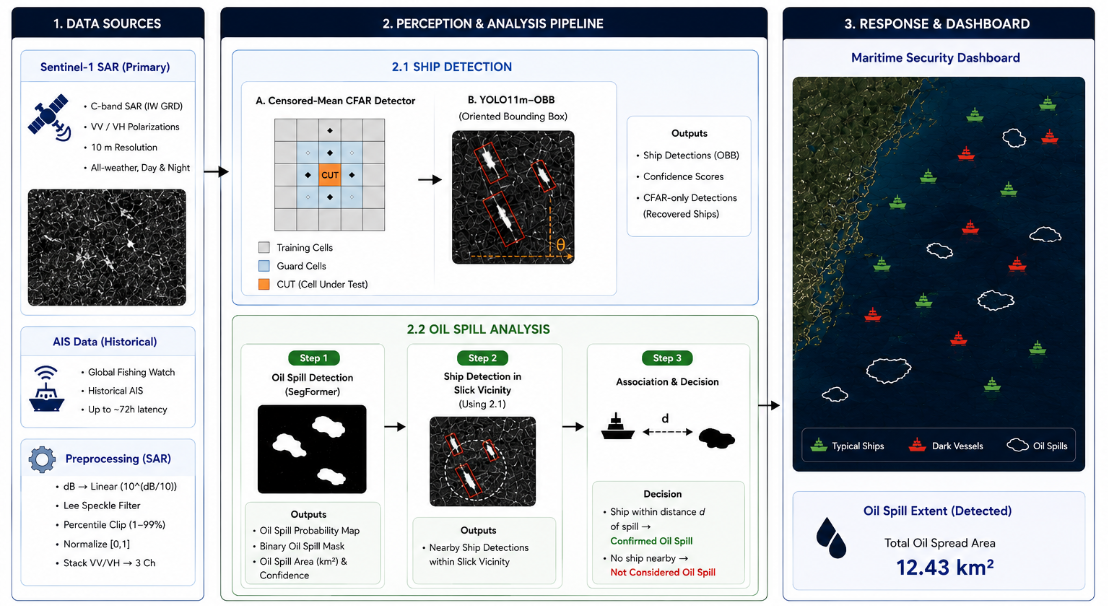
\includegraphics[width=0.78\textwidth]{methodology.png}
  \caption{End-to-end architecture of the proposed framework. Left: data sources---Sentinel-1 IW GRD imagery as the primary sensor, historical AIS, and the SAR preprocessing chain, of which each perception branch applies the variant matched to its own training distribution (Section~\ref{subsec:data}). Centre: the perception and analysis pipeline---ship detection by censored-mean CFAR fused with YOLO11m-OBB, followed by SegFormer oil-spill analysis and slick-to-vessel association. Right: the response layer, where georeferenced AIS-matched and dark-vessel detections and the measured oil-spill extent drive the maritime-security dashboard.}
  \label{fig:methodology}
\end{figure*}

\begin{table}[p]
\caption{\textbf{Datasets used in the framework: HRSID for vessel detection and the three-part Sentinel-1 oil-spill dataset for segmentation, with Parts~I+II forming the train/validation pool and Part~III held out for the robustness analysis.}}
\label{tab:datasets}
\centering
\renewcommand{\arraystretch}{1.2}
\begin{tabularx}{\columnwidth}{|p{2.3cm}|X|}
\hline
\textbf{Dataset} & \textbf{Task, description, and role} \\
\hline
HRSID~\cite{4} & Vessel detection. High-resolution SAR ship chips ($5{,}604$ images, $16{,}951$ instances, $800\times800$\,px); $3{,}642$ train / $1{,}962$ test, plus $400$ pure-background negatives. \\
\hline
Trujillo-Acatitla \textit{et al.}~\cite{6} & Oil segmentation. Sentinel-1 C-band dual-pol (VV/VH), $\sigma^0$ in dB, $2048\times2048$\,px; Parts~I+II for train/validation, Part~III held out as the test set. \\
\hline
\end{tabularx}
\end{table}

\begin{table*}[p]
\caption{\textbf{Vessel-detection benchmark on the HRSID test set ($1{,}962$ images, $5{,}922$ ship instances, $50$ epochs on dual T4 GPUs). $F_1$ is the harmonic mean of precision and recall. Best per column in bold.}}
\label{tab:ships}
\centering
\renewcommand{\arraystretch}{1.2}
\begin{tabularx}{\textwidth}{|X|c|c|c|c|c|c|}
\hline
\textbf{Model} & \textbf{Precision} & \textbf{Recall} & \textbf{$F_1$} & \textbf{mAP@50} & \textbf{mAP@50-95} & \textbf{Train time} \\
\hline
YOLOv8m (2023, horizontal)   & 0.913 & 0.822 & 0.865 & 0.910 & 0.669 & 2.03\,h \\
\hline
YOLO26m (2026, horizontal)   & \textbf{0.926} & 0.802 & 0.860 & 0.908 & 0.671 & 2.67\,h \\
\hline
YOLO11m-OBB (2024, oriented) & 0.920 & \textbf{0.873} & \textbf{0.896} & \textbf{0.938} & \textbf{0.688} & 2.42\,h \\
\hline
\end{tabularx}
\end{table*}

\begin{figure}[p]
  \centering
  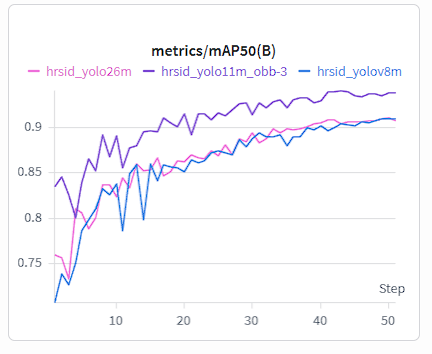
\includegraphics[width=\columnwidth]{ship_map50.png}
  \caption{Validation mAP@50 over $50$ training epochs for the three vessel detectors on HRSID. YOLO11m-OBB maintains a clear margin over the horizontal-box models YOLOv8m and YOLO26m for essentially the entire run, finishing at $0.938$ against $0.910$ and $0.908$ respectively---the oriented-box geometric prior, not architectural recency, drives the gap.}
  \label{fig:shipcurves}
\end{figure}

\begin{figure}[p]
  \centering
  \includegraphics[width=\columnwidth]{fig_ship_detection.png}
  \caption{YOLO11m-OBB oriented-box predictions on SAR imagery. The rotated boxes fit elongated vessels at their true headings, excluding the speckle-dominated sea background that an axis-aligned box around the same target would enclose.}
  \label{fig:shippred}
\end{figure}

\begin{table}[p]
\caption{\textbf{Vessel-detection counts on a dense Sentinel-1 IW scene (Singapore Eastern Anchorage, $\sim$10\,m/px). The fusion keeps CFAR's recall while attaching oriented geometry to the $141$ vessels the learned detector resolves.}}
\label{tab:cfar}
\centering
\renewcommand{\arraystretch}{1.2}
\begin{tabularx}{\columnwidth}{|p{2.4cm}|c|X|}
\hline
\textbf{Method} & \textbf{Detected} & \textbf{Characteristics} \\
\hline
Censored-mean CFAR ($\alpha=20$) & $257$ & Training-free, resolution-agnostic, high recall \\
\hline
CFAR\,$\rightarrow$\,YOLO fusion & $141{+}116$ & Recall of CFAR + oriented geometry ($141$ confirmed OBB, $116$ CFAR-only) \\
\hline
YOLO11m-OBB standalone & $0$--$165$ & Inconsistent; HRSID$\rightarrow$10\,m domain gap \\
\hline
\end{tabularx}
\end{table}

\begin{figure}[p]
  \centering
  \includegraphics[width=\columnwidth]{fig_cfar_malacca.png}
  \caption{Censored-mean CFAR detections ($\alpha=20$) on a Strait of Malacca Sentinel-1 IW scene ($\sim$10\,m/px). Open-water vessels are recovered without any training data, while the $-18$\,dB land mask suppresses coastal returns; this is the resolution regime in which the HRSID-trained network alone becomes unreliable.}
  \label{fig:cfarpred}
\end{figure}

\begin{table*}[p]
\caption{\textbf{Oil-spill segmentation results: validation OilIoU on the Parts~I+II split (primary benchmark) and figures on the held-out Part~III stress set ($450$ scenes, one third look-alikes; $\tau=0.5$). Best per column in bold.}}
\label{tab:oil}
\centering
\renewcommand{\arraystretch}{1.2}
\begin{tabularx}{\textwidth}{|X|c|c|c|c|c|c|}
\hline
\textbf{Model} & \textbf{Params} & \textbf{val OilIoU} & \textbf{test OilIoU} & \textbf{test mIoU} & \textbf{val$\rightarrow$test} & \textbf{Train time} \\
\hline
U-Net        & ---     & 0.750 & 0.369 & 0.673 & $-0.381$ & 44\,m \\
\hline
DeepLabV3+   & 26.7\,M & 0.773 & 0.356 & 0.667 & $-0.417$ & 45\,m \\
\hline
SegFormer-b4 & 64.0\,M & \textbf{0.799} & 0.481 & \textbf{0.731} & $-0.318$ & 1\,h\,22\,m \\
\hline
SegFormer-b5 & 82.0\,M & 0.795 & \textbf{0.484} & --- & $\mathbf{-0.311}$ & 1\,h\,15\,m \\
\hline
\end{tabularx}
\end{table*}

\begin{figure}[p]
  \centering
  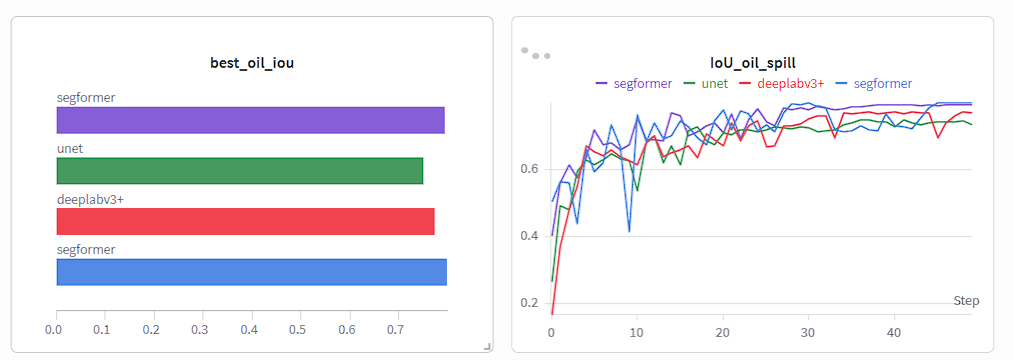
\includegraphics[width=\columnwidth]{oil_metrics.png}
  \caption{Oil-segmentation training summary: best validation oil-class IoU per run (left) and validation oil-class IoU over $50$ training epochs (right). Both SegFormer variants converge above the DeepLabV3+ and U-Net baselines.}
  \label{fig:oilcurves}
\end{figure}

\begin{figure*}[p]
  \centering
  \includegraphics[width=\textwidth]{fig_oil_segmentation.png}
  \caption{SegFormer oil-spill segmentation on a held-out Part~III scene, compared against the reference mask. The predicted mask follows the slick outline closely while rejecting the surrounding sea, illustrating the whole-scene-resize inference path of Section~\ref{subsec:oil}.}
  \label{fig:oilpred}
\end{figure*}

\begin{figure*}[p]
  \centering
  \includegraphics[width=\textwidth]{fig_dashboard.png}
  \caption{Integrated dashboard output for a Sentinel-1 scene. The map pane overlays the vessel detections (AIS-matched and dark) and oil-slick polygons on the SAR backdrop, while the side panel reports scene metadata, coverage, detection counts, and the measured oil-spill extent (area, spread, and patch count).}
  \label{fig:dashboard}
\end{figure*}

\EOD

\end{document}
